% Updated in February 2016 by Hwann-Tzong Chen
% Updated in May 2014 by Hideo Saito
% Updated in March 2012 by Yasuyuki Matsushita
% Updated in April 2002 by Antje Endemann, ...., and in March 2010 by Reinhard Klette
% Based on CVPR 07 and LNCS style, with modifications by DAF, AZ and elle 2008, AA 2010, ACCV 2010

\documentclass[runningheads]{llncs}
\usepackage{graphicx}
\usepackage{amsmath,amssymb} % define this before the line numbering.
\usepackage{ruler}
\usepackage{color}
\usepackage{subfigure}
\usepackage{mathrsfs}
\usepackage[marginal]{footmisc}
\renewcommand{\thefootnote}{}
\usepackage{bm}
\usepackage{booktabs}
\usepackage{array}
\usepackage{url}
\newcommand{\PreserveBackslash}[1]{\let\temp=\\#1\let\\=\temp}
\newcolumntype{C}[1]{>{\PreserveBackslash\centering}p{#1}}
\newcolumntype{R}[1]{>{\PreserveBackslash\raggedleft}p{#1}}
\newcolumntype{L}[1]{>{\PreserveBackslash\raggedright}p{#1}}
%===========================================================
\begin{document}
\pagestyle{headings}
\mainmatter

\def\ACCV16SubNumber{663}  % Insert your submission number here

%===========================================================
\title{HF-FCN: Hierarchically Fused Fully Convolutional Network for Robust Building Extraction} % Replace with your title
%\subtitle{Robust Building Extraction from Large-scale Aerial Scene with  hierarchically fused Fully Convolutional Network}
\titlerunning{ACCV-16 submission ID \ACCV16SubNumber}
\authorrunning{ACCV-16 submission ID \ACCV16SubNumber}

\author{Anonymous ACCV 2016 submission}
\institute{Paper ID \ACCV16SubNumber}

\maketitle
%===========================================================
\begin{abstract}
  Currently, automatic building extraction from remote sensing images plays an important role in  a diverse range of applications. However, it is significantly  challenging to extract arbitrary-size buildings with large variant appearances or occlusions. To tackle these problems, we propose a robust system employing a novel hierarchically fused fully convolutional network (HF-FCN), which effectively integrates the information generated from a group of neurons with multi-scale receptive fields. Our architecture can take  whole aerial images as inputs without warping or cropping and output building map directly. The experiment results tested on a publicly available aerial imagery dataset prove that our proposed methodology surpass the performance of state-of-the-art method and  significantly reduce time cost.

\end{abstract}

%===========================================================
\section{Introduction}
   With the rapid development of remote sensing technologies and popularization of geospatial related commercial softwares, very high resolution satellite images are easily accessible. These valuable data provide a huge fuel for interpreting real terrestrial scenes. The building rooftop is one of the most important type of terrestrial objects because it is essential for a wide range of technologies, such as, urban planning, automated map making, 3D city modelling, disaster assessment, military reconnaissance, etc. However, it is very costly and time-consuming to manually delineate the footprint of buildings even for human experts. 
   
   In recent decades, many researchers have made massive attempts to extract buildings automatically. Much of the past works define criteria according to the particular  characteristics of rooftop, such as, polygonal boundary \cite{noronha2001detection,nosrati2009novel,izadi2012three,wang2015efficient}, homogeneous color or texture \cite{cote2013automatic}, surrounding shadow \cite{B2008Building,ok2013automated,chen2014shadow,ngoautomatic}, and their combinations \cite{baluyan2013novel,li2015robust}. However, such approaches are weakly capable of handling real-world data because hand-coded rules or probability models learned from small samples are much dependent on data. For example, they assume that profile of buildings is polygon while the shape of stadiums always is circle or oval. For the sake of deploying a practical building extraction system, Mnih \cite{Mnih2013Machine} created a huge publicly dataset including large-scale aerial images and corresponding human-labeled maps, and proposed a patch-based convolutional neural network to extract location of objects automatically. Based on Mnih's work, Saito \textit{et al}. \cite{Saito2016Multiple} improved the performance further by developing two effective techniques. Though these methods achieve high performance, they still have limited ability to deal with two often appearing cases: (1) Buildings are  occluded by shadows or trees. (2) Buildings possess moderately variant appearances. 
      
   Mapping buildings from aerial image is essentially a problem of semantic segmentation. Recent work suggests a number of methods in processing natural images. Long \textit{et al.} \cite{Long2014Fully} firstly proposed a effective architecture for semantic image segmentation, namely, fully convolutional network (FCN).  
%   the coarse predictions from a late stage are upsampled and integrated with predictions from previous stage to yield finer ones, the whole procedure is repeated in this fashion until reaching a desired output. 
Chen \textit{et al.} \cite{chen14semantic} presented a system which combines the responses at the final convolutional layer with a fully connected conditional random field (CRF). The system is able to localize segment boundaries at a quite high level of accuracy. Zheng \textit{et al.} \cite{Zheng2015Conditional} introduced an end-to-end network  which integrates CRF with CNNs to avoid off-line post-processing  for object delineation. Noh \textit{et al.} \cite{Noh2015Learning} applied a deconvolution network to each proposal in a input image, and construct the final semantic segmentation map by combining the results from all proposals in a simple manner.
     
   Although these methods show promise in segmenting natural images, they have components not suited for building extraction. Firstly, buildings are frequently occluded by shadows or trees (see Fig.\ref{fig:AerialImages} (a)). It is challengable to delineate building boundaries even for human experts. Though some literatures \cite{chen14semantic,Zheng2015Conditional} achieve excellent performance in processing boundary of natural image, neither of them reported that they have strong ability in handling occlusions. Secondly, buildings have significantly variant appearances even in a single one. (see Fig.\ref{fig:AerialImages} (b)). Moreover, a number of buildings are very close to the plot on the ground or road (see Fig.\ref{fig:AerialImages} (c)). Based on our observation, there are few such samples emerge in PASACAL VOC 2012 \cite{pascal-voc-2012} dataset. Last but not the least, the size of objects in a remote sensing image is in a wide range. For example, some images include a large number of tiny buildings (see Fig.\ref{fig:AerialImages} (d)) and some ones are composed of moderate quantity of small-scale rooftops and a few  large-scale rooftops. On account of low resolution (one-eighth resolution of input image) of output from \cite{Long2014Fully}, precise structures are sacrificed severely. Noh \textit{et al.} \cite{Noh2015Learning} claimed  it handles objects in multiple scales, but it only suitable to multi-classes object segmentation. 

%It is reported that \cite{Long2014Fully} have limited ability to locate small objects.

\begin{figure}
\centering
\label{fig:AerialImages}
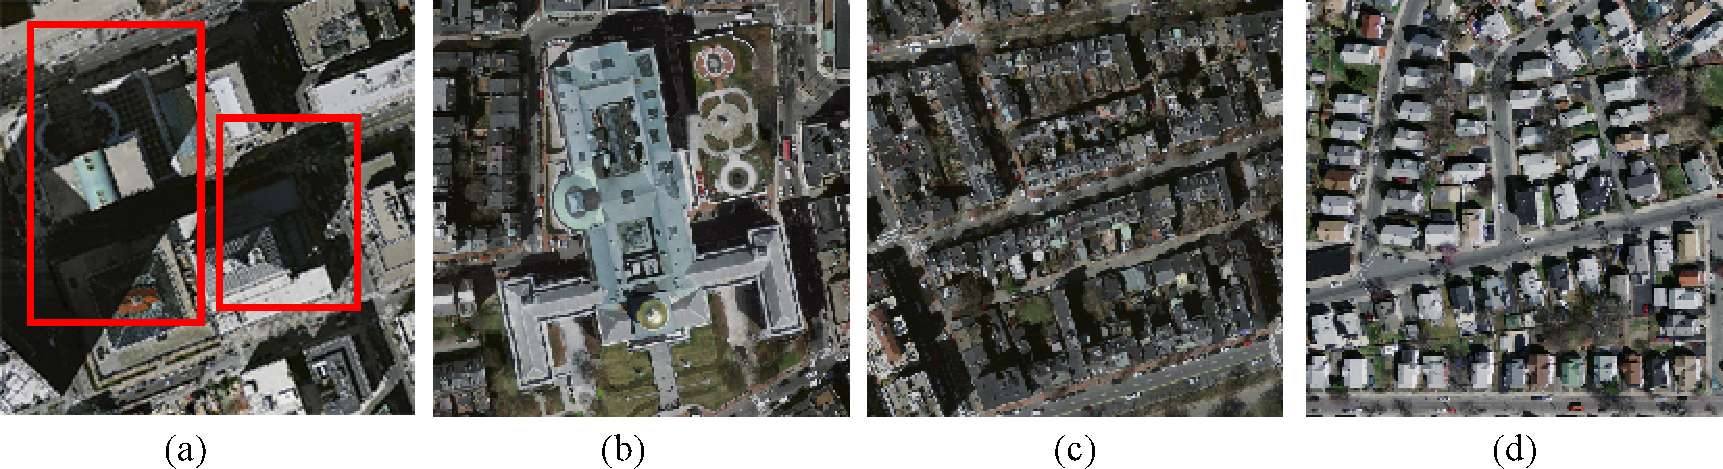
\includegraphics[width=120mm]{AerialImages}
\caption{Examples of aerial image. (a) Occlusions (shown in red rectangle). (b) Variant appearances. (c) Low contrast. (d) A large number of tiny buildings. }
\end{figure}      
            
  Here, we present a robust building extraction system by developing a hierarchically fused fully convolutional network (HF-FCN) trained on a publicly available large aerial imagery dataset \cite{Mnih2013Machine}. In our architecture (HF-FCN), we design a new scheme to integrate multi-level semantic information generated from convolutional layers with a group of incremental receptive fields. Incremental sized receptive fields are able to capture context information in different neighbourhood sizes. Therefore, it is more effective to handling buildings with arbitrary sizes, variant appearances or occlusions. Compared with \cite{Mnih2013Machine,Saito2016Multiple}, overlapped cropping and model averaging are not required for HF-FCN. It takes whole images as inputs, and directly outputs segmentation maps by one pass of forward propagation. Hence, our system decreases the computation complexity significantly. In conclusion, our contributions include two aspects: (1) A new architecture is developed for building extraction, which has a strong ability in processing appearance variations,  varying sizes and occlusions. Meanwhile, the overall accuracy  also exceeds state-of-the-art \cite{Saito2016Multiple}. (2) Our approach leads to a notable reduction of computation cost  compared with traditional solutions.
  
  
   The rest of this article is organized as follows. In Section \ref{section:relatedworks}, we summarize main   methods for building extraction. Section \ref{section:systemoverview} provides details of our neural network architecture and formulation of building extraction problem. Section \ref{section:experiments} introduces the dataset and training strategies of our proposed network, and then we compare our results with two patch-based methods using the three types of criteria. In Section \ref{section:conclusions}, we discuss the experimental results and summarize whole article. 
   
   
\section{Related Work}
\label{section:relatedworks}
   In previous literatures, one popular way of extracting buildings is employing their shape information. It is observed that rooftops have more regular shapes, which usually are rectangular or combinations of several rectangles. Several studies   \cite{noronha2001detection,nosrati2009novel,izadi2012three,wang2015efficient} exploited a graph-based search to establish a set of rooftop hypotheses through examining the relationships of lines and line intersections, and then removed the fake hypotheses using a series of criteria. Cote and Saeedi \cite{cote2013automatic} generated rooftop outline from selected corners in  multiple color and color-invariance spaces, further refined to fit the best possible boundaries through level-set curve evolution. Though these geometric primitives based methods achieve good performance in high contract remote sensing imagery, they suffer from three  shortcomings. Firstly, they lack the ability of detecting arbitrarily shaped building rooftop. Secondly, they fail to  extract credible geometric features in buildings with inhomogeneous color distribution or low contrast with surroundings. Thirdly, it is time-consuming to process large-scale scenes because of their high computational complexity.	
   
   Apart from using shape information, spectral information is a distinctive feature for  terrestrial object extraction. For instance, shadows are commonly dark grey or black, vegetations are usually green or yellow with particular textures, and main roads are dim gray in most cases. According to these prior knowledge, Ghaffarian \textit{et al.} \cite{ghaffarian2014automaticPFICA} split aerial scenes into three components (respectively, shadows and the vegetation, roads and the bare soil, buildings) using a group of manually established rules. Afterwards, a purposive fast independent component analysis (PFastICA) technique is employed to separate building area from remote sensing image. However, their results are significantly sensitive to parameter choice. A feasible alternative strategy is to learn the appearance representation using  supervised learning algorithm. A number of authors \cite{chen2014shadow,ngoautomatic,baluyan2013novel,dornaika2015object} designed a similar framework. Firstly, an aerial image is divided into superpixels using  a certain over-segmentation algorithm. Secondly, hand-crafted features, such as, color histograms or local binary patterns (LBP), are extracted from each over-segmented regions. Finally, each region is classified using machine learning tools and a gallery of training descriptors.  Because it's inevitable for machine learning method to mislabel regions with similar appearance, additional information is utilized to refine previous results. Ngo \textit{et
al.} \cite{ngoautomatic} removed false rooftops using a assumption that buildings are surrounded by shadows because of illumination. Baluyan et al. \cite{baluyan2013novel} devised a ``histogram method" to detect missed rooftops. Li \textit{et al.} \cite{li2015robust} selected probable rooftops after pruning out blobs using shadows, light direction, a series of shape criteria, and then these rooftops is refined by high order conditional random field. The drawbacks of these algorithms are threefold. (1) It is problematic to recognize a over-segmented region as part of buildings because terrestrial objects have huge variant appearances in real aerial scene. (2) Hand-craft features are sensitive to input data, therefore, it is not robust to process large-scale remote sensing images. (3) Additional information is unreliable. For instance, some low buildings have no shadow in its neighbourhood, and some buildings have unique structures which are not satisfied to hand-coded criteria. 

    As mentioned above, traditional methods are weakly capable of adapting to real scenes with huge variant appearances, occlusions or low contrast. Our method does not design image features manually, on the contrary, building features are directly learned from a mass of real data 
using deep neural networks. Therefore, our algorithm is more robust to  extract buildings in real scenes.  Mnih, a pioneer,  presented a patch-based framework for learning to label aerial images \cite{Mnih2013Machine}. A  neural network architecture is carefully designed for predicting buildings in aerial imagery, and the output of this network is processed by conditional random fields (CRFs). Satito \textit{et al.} \cite{Saito2016Multiple} improved Mnih's networks for extracting multiple kinds of objects simultaneously, two techniques consisting of model averaging with spatial displacement (MA) and channel-wise inhibited softmax (CIS) are introduced to enhance the  performance. However, these methods need to crop test image into a fixed size, which not only increases the time cost, but also breaks the integrity of buildings. Our system takes whole images as inputs without overlapped cropping or wrapping and directly outputs labelling images. It is much beneficial  to preserve the whole structure of buildings and shorten computation time.


%    For example, they obtain bad performance for large-size or occluded buildings (see Fig. \ref{fig:BadResults}) and cost about 9s for 1500 $\times$ 1500 image without model averaging. 
   
% Recently,  have been widely deployed in general image segmentation or scene labelling tasks.
%===========================================================
\section{System Overview} 
\label{section:systemoverview}
   In this section, we introduce a hierarchically fused fully convolutional network (HF-FCN) for extracting rooftops, and then formulate our problem and loss function.
         
\subsection{Network Architecture} 
   We design our network based on VGG16 Net \cite{Simonyan2014Very} and make some modifications. The reasons for choose VGG16 Net are two-fold: (1) It has great depth (16 convolutional layers), and multiple stages (five 2-stride down-sampling layers). We can acquire enough multi-level information from different stages and convolutional layers. (2) Network parameters pre-trained on very large image dataset (ImageNet) are helpful for initializing our network  because our aerial data is essentially optical imagery.  The modifications are listed as follows: (1) Two fully connected layer \textit{fc6, fc7} and fifth pooling layer are cut, because they are at 1/32 of input resolution with the consequence that the interpolated prediction map will be too fuzzy to utilize. Meanwhile, the number of neurons in \textit{fc6, fc7} is too large to cost intensive computation. (2) Feature maps from each convolutional layer in trimmed VGG16 Net (denote as Level 1) are fed into a convolutional layer with a filter of kernel size of 1$\times$1. The outputs of these convolutional layers are upsampled and cropped to the same size of input image (denote as Level 2). Upsampling is implemented via deconvolution which is initialized by bilinear interpolation.  Finally, all the  feature maps in Level 2 are stacked and put into a convolutional layer with  a filter of kernel size of 1$\times$1  to yield final predicted map (denote as Level 3). (3) The  size of  feature map in last stage of Level 1 is 1/16 of input image, it is too small to use. Thus, we apply a popular trick that  input images are padded with all-zero band to enlarge the size of feature maps. Our architecture is shown in Fig. \ref{fig:hierarchicalFCN}.
 
\begin{figure}
\centering
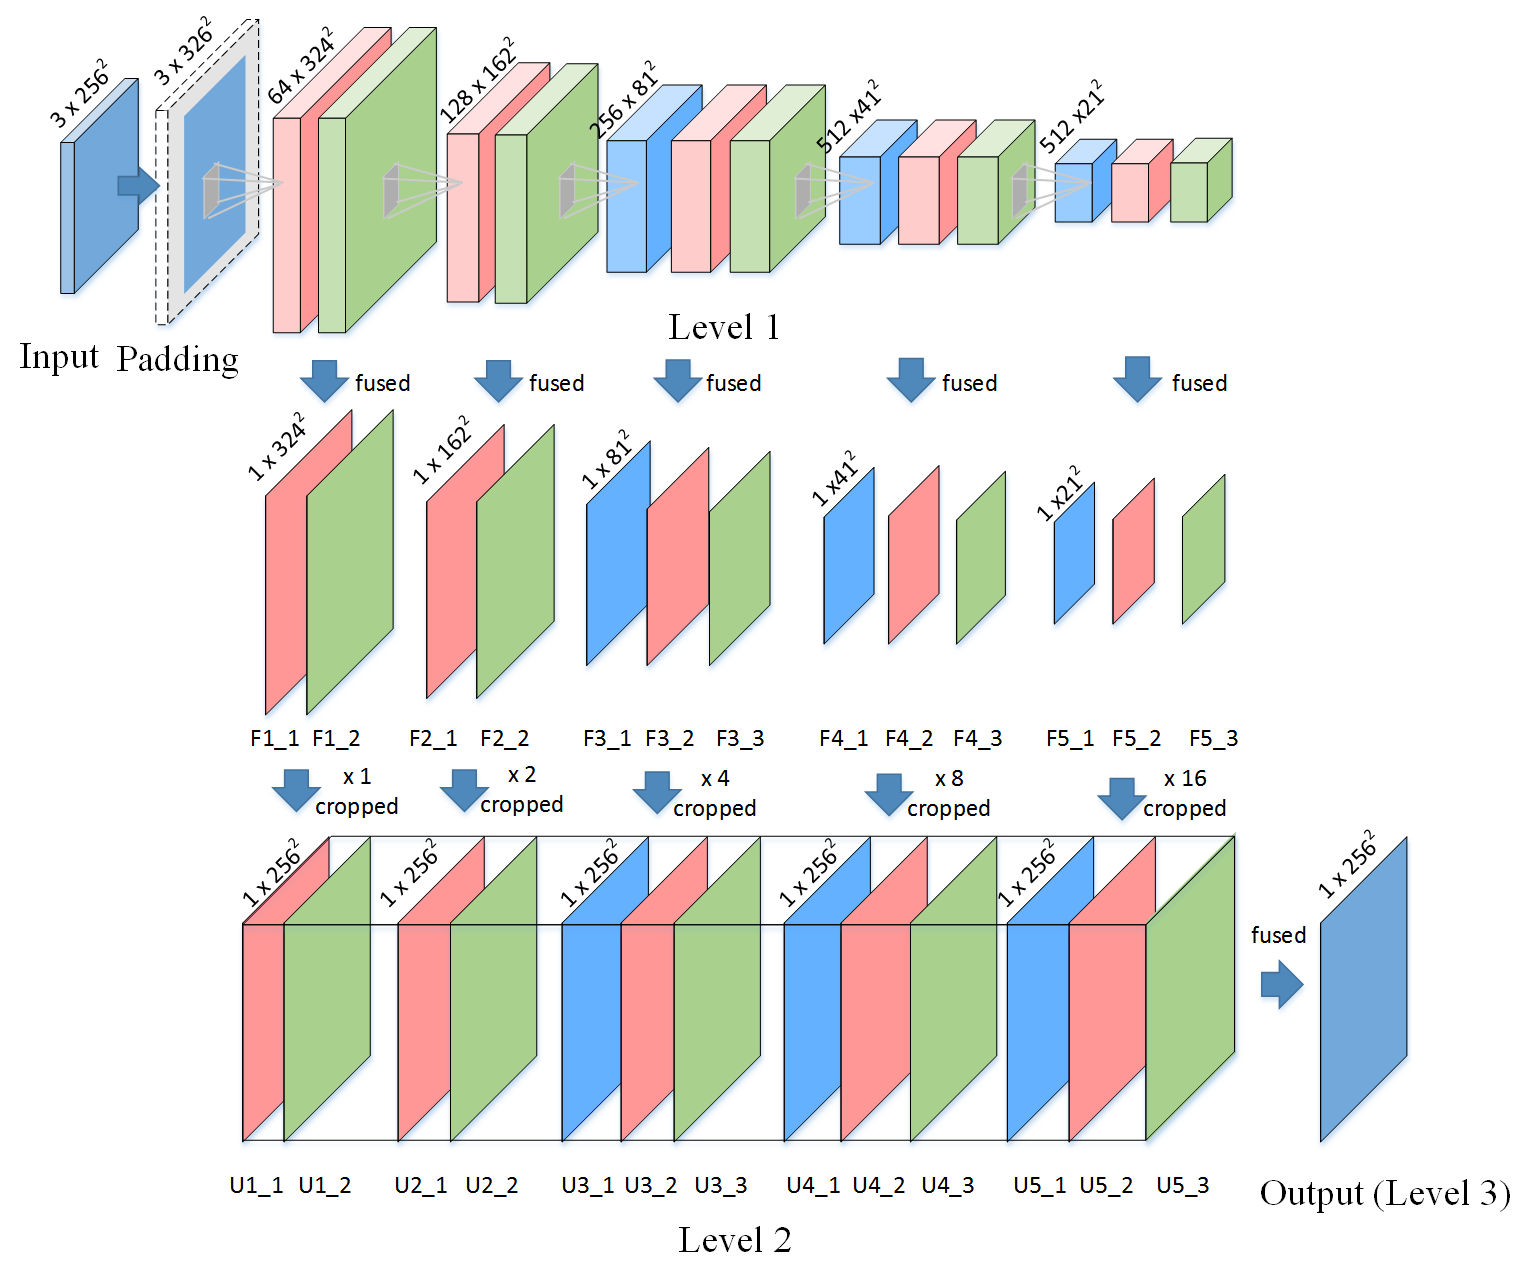
\includegraphics[height=85mm]{hierarchicalFCN9}
\caption{Our network architecture.}
\label{fig:hierarchicalFCN}
\end{figure}

   \begin{table}	
	\centering 
	\caption{The receptive field (rf) and stride size of Level 2 in our architecture.}	
 	\begin{tabular}{C{1cm}|*{16}{C{0.74cm}}} 
	\hline
	layer & F1$\_$1 & F1$\_$2  & F2$\_$1  & F2$\_$2  & F3$\_$1  & F3$\_$2  & F3$\_$3  & F4$\_$1  &   F4$\_$2  & F4$\_$3  & F5$\_$1 & F5$\_$2  &F5$\_$3 \\
	\hline
    rf size & 3 & 5  & 10 & 14  & 24  & 32  & 40  & 60  & 76  & 92 & 124  & 164  & 196 \\
	\hline
	stride & 1 & 1   & 2  & 2  & 4  & 4  & 4  &8  & 8  & 8  & 16  & 16  & 16 \\
	\hline
    \end{tabular}
    \label{tab:receptivefield} 
   \end{table}         
    
   In Level 2 of our architecture, feature maps with increasing  receptive field (see Table \ref{tab:receptivefield}) capture local information in different neighbourhood sizes and at different semantic levels. Therefore, if we integrate all these information together, it is helpful for extracting buildings with variant appearances or occlusions. We take a concrete instance  to show how HF-FCN works for such cases. In this case, U1$\_$1 with small receptive field  generates fine spatial resolution and responds to low level features like edges and corners (see Fig. \ref{fig:featuremapsofHF-FCN}(b)). U1$\_$2 functions like over-segmentation algorithm to grouping pixels with similar color or texture into a subregion (see Fig. \ref{fig:featuremapsofHF-FCN}(c)). In U2$\_$1, color information is disappear, shape information is augmented (see Fig. \ref{fig:featuremapsofHF-FCN}(d)). In U3$\_$3, it is surprised that  regions with significantly varying appearance are merged into a integrated building by considering some unknown high level features (see Fig. \ref{fig:featuremapsofHF-FCN}(e)). In U4$\_$2 and U5$\_$2, our network learned strong semantic knowledge  to distinguish dark rooftops with dim shadows and dark-green water (see Fig. \ref{fig:featuremapsofHF-FCN}(f)(g)). In Level 3, we show that HF-FCN obtains reliable prediction by combining multi-level semantic information and  spatial information (see Fig. \ref{fig:featuremapsofHF-FCN}(h)). 

\begin{figure}
\centering
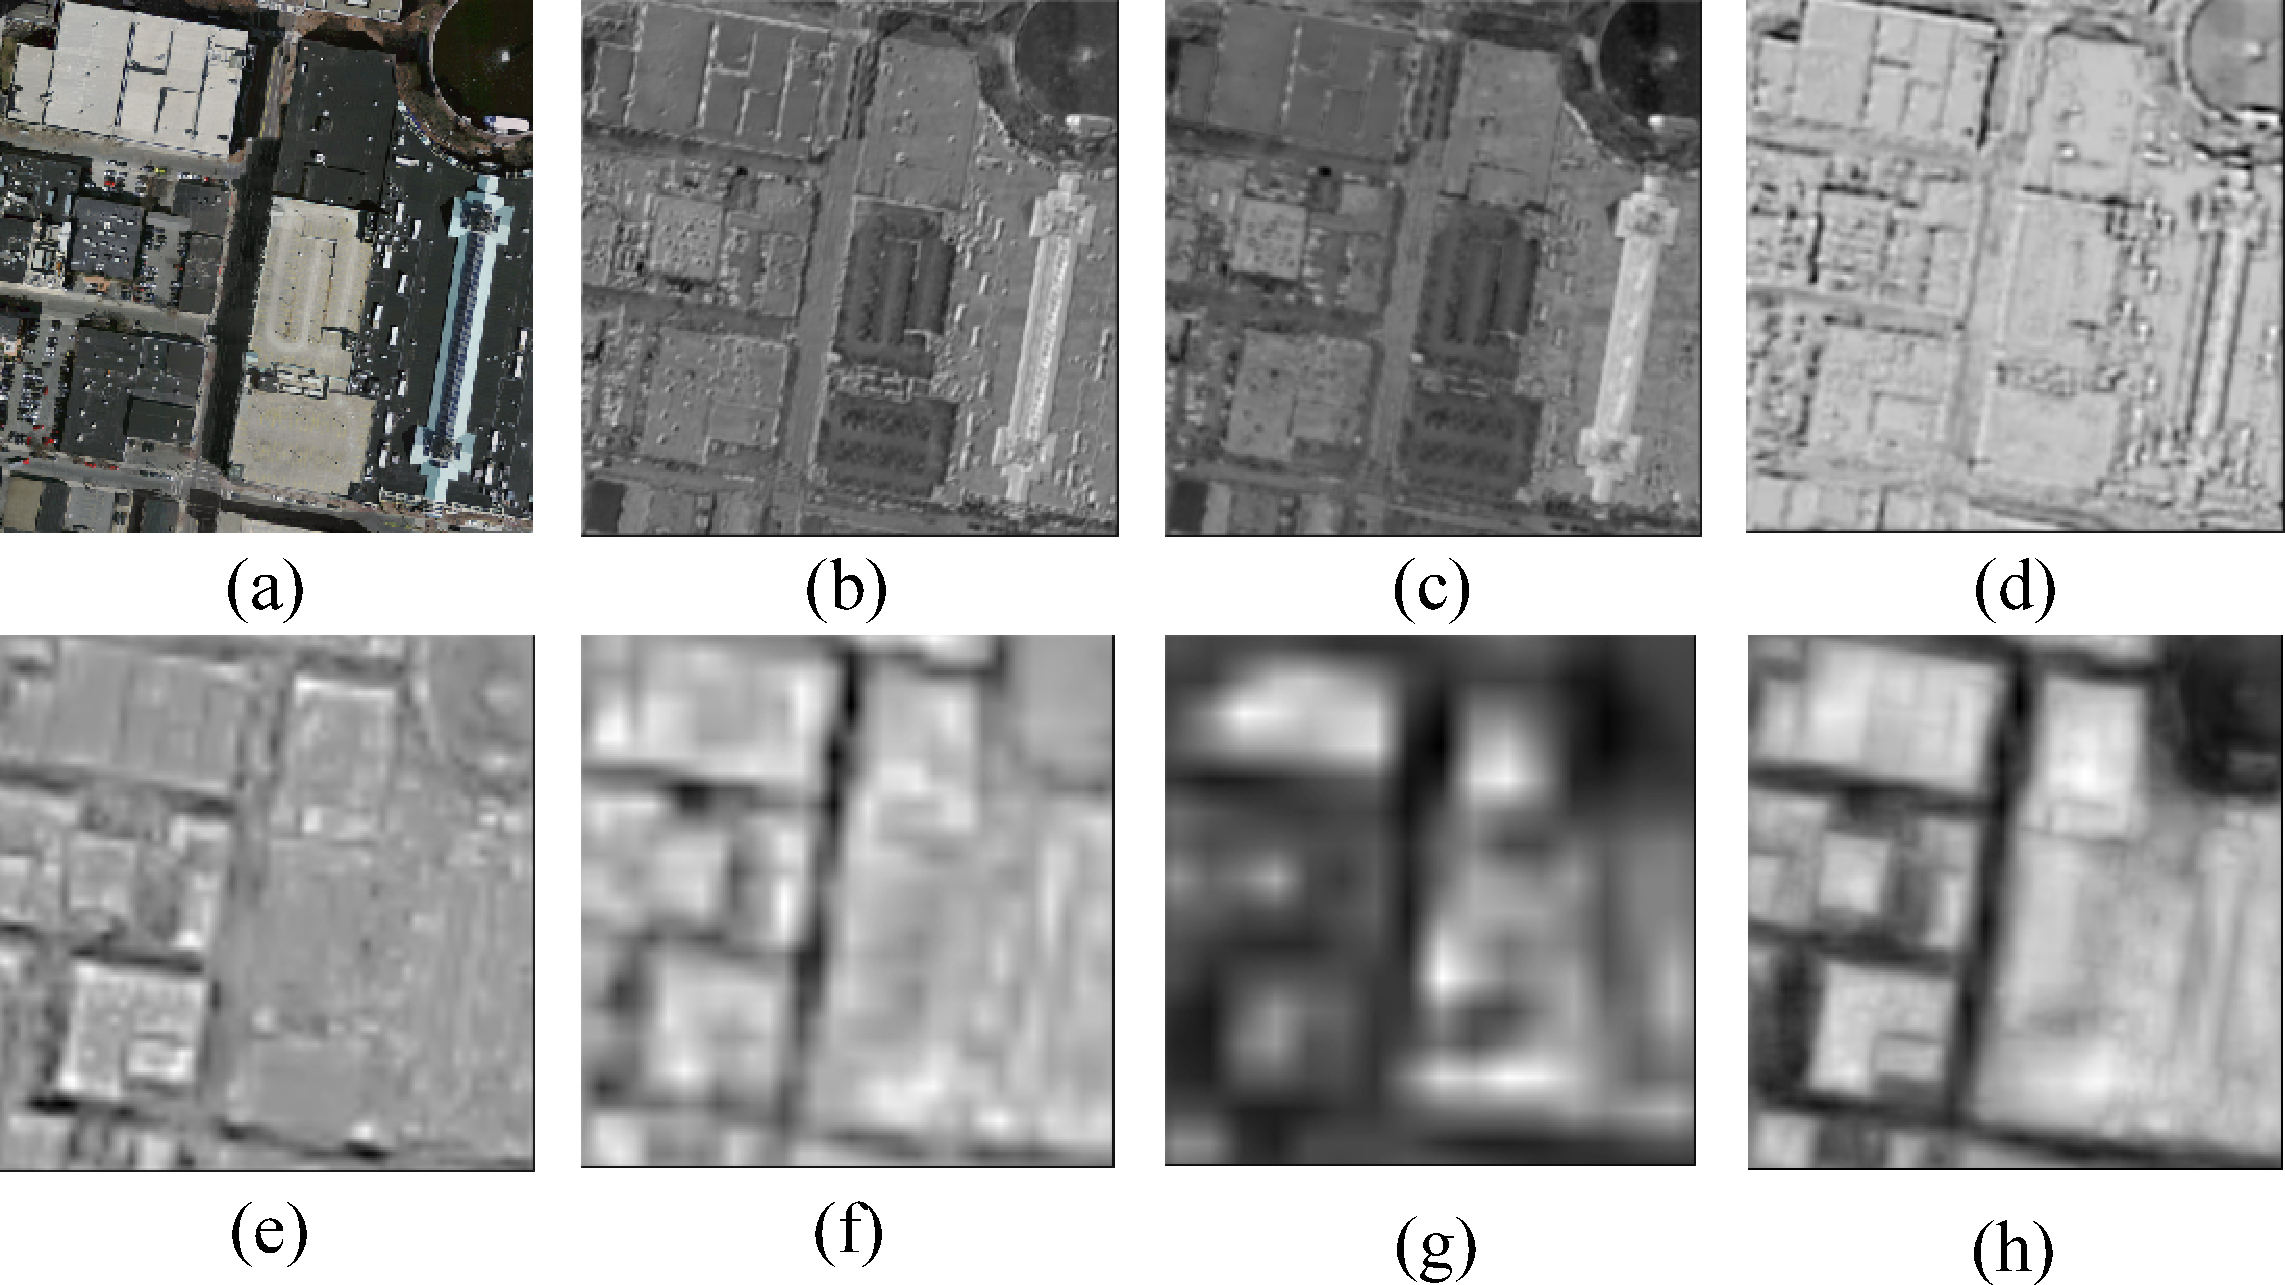
\includegraphics[width=120mm]{featuremaps}
\caption{(a) Input aerial image. (b - g) Feature maps generated from U1$\_$1, U1$\_$2, U2$\_$1, U3$\_$3, U4$\_$2, U5$\_$2, respectively. (h) Predicted labelling map.}
\label{fig:featuremapsofHF-FCN}
\end{figure}

%   In VGG16 Net, 
%   For instance, the first stage generate low level semantic information, such as, regions with similar color or texture, and fine spatial resolution. On the contrary, the last stage outputs strong semantic features but coarse map
%   
%   There are three reasons that FCN-8s is not appropriate methods for building extraction. (1) \textbf{The output of 32 stride layers, including convolutionalized \textit{fc6, fc7} and fifth pooling layer, } (2) The output from FCN-8s is at one-eight of the input resolution. It is not dense enough for very high resolution remote sensing image. Though FCN4s and FCN2s can increase the resolution, they have little help for improving performance. Defective fusion strategy is the most likely reason. On the one hand, in \cite{Long2014Fully}, the coarse predictions from a late stage are upsampled and combined with prediction from its preceding stage using simple sum operation. (3) \textbf{ For instance, in FCN-8s,
%   
% There are two main considerations for choosing hierarchy architecture. Firstly,  buildings especially with large-size have variant appearancess or occlusions.   
   
%\subsection{Architecture Alternatives} 
%In this section, we firstly introduce a well-known semantic segmentation network, called fully convolutional network(FCN)\cite{Long2014Fully}. We attempt to extract footprints of building  using  architecture proposed by author and two modified versions. Our experiments show that these networks are not enough to accomplish building  extraction task. 
%	In our experiments, we first directly apply the FCN-8s to extract building rooftop by replacing the loss function with sigmoid cross-entropy loss. In order to achieving better performance, the network is extended to FCN-4s, FCN-2s. Our experiments show that FCN-4s and FCN-2s get the best performance with overall recall of 70.19 $\%$ in precision recall breakeven point. According to our results, the first row of Fig. \ref{fig:FCN4s-results} indicates that FCN-4s has less ability to handle  objects with small size. The second row of Fig. \ref{fig:FCN4s-results} shows that it is hard for FCN to discriminate buildings with ground if their color is similar. To overcome these drawbacks, a improved FCN is introduced in next section. 
%	
%\begin{figure}
%\centering
%\subfigure[]{	
%	\label{fig:InputImage}
%	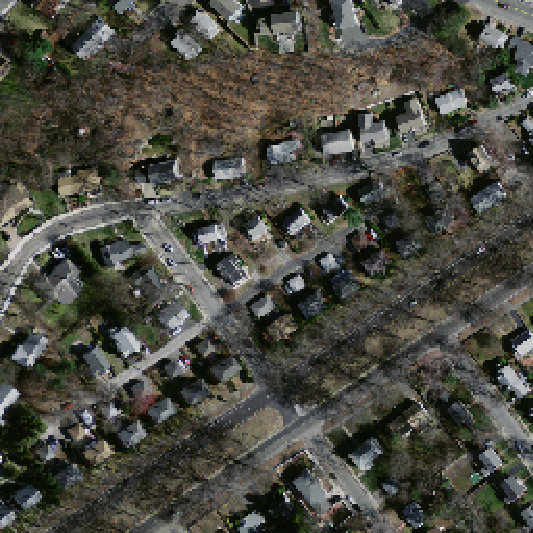
\includegraphics[width=35mm]{FCN4s-results-Input(a)}}
%\subfigure[]{
%	\label{fig:GroundTruth}
%	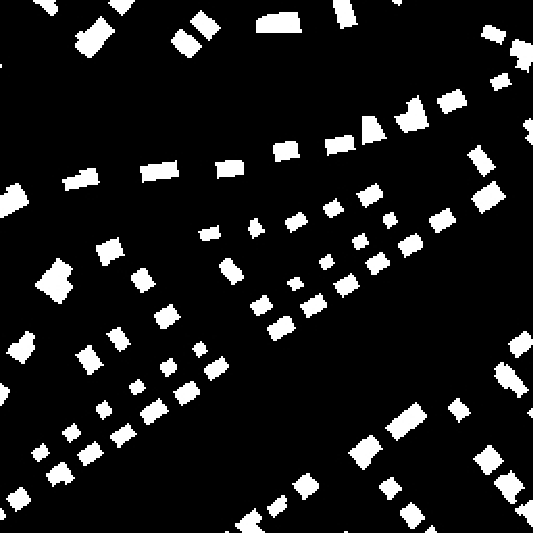
\includegraphics[width=35mm]{FCN4s-results-GT(b)}}
%\subfigure[]{
%	\label{fig:FCN-4s}
%	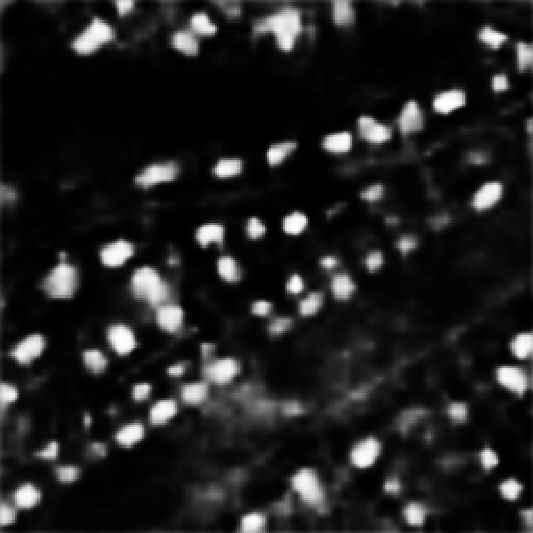
\includegraphics[width=35mm]{FCN4s-results-Prediction(c)}}
%\subfigure[]{	
%	\label{fig:InputImage}
%	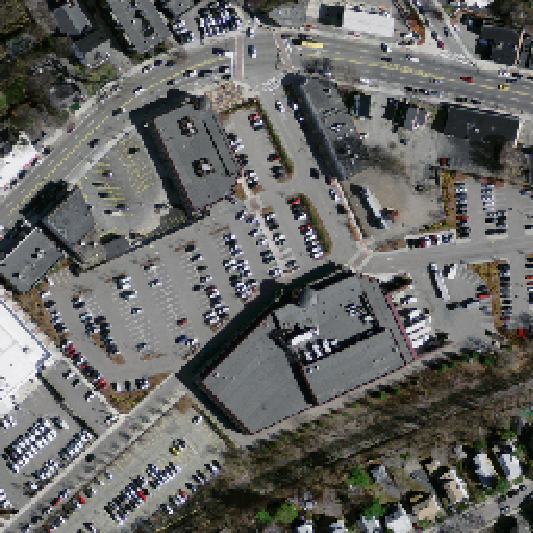
\includegraphics[width=35mm]{FCN4s-results-Input(d)}}
%\subfigure[]{
%	\label{fig:GroundTruth}
%	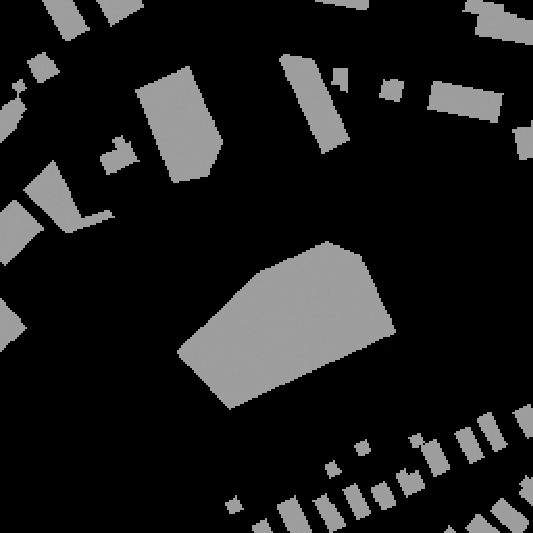
\includegraphics[width=35mm]{FCN4s-results-GT(e)}}
%\subfigure[]{
%	\label{fig:FCN-4s}
%	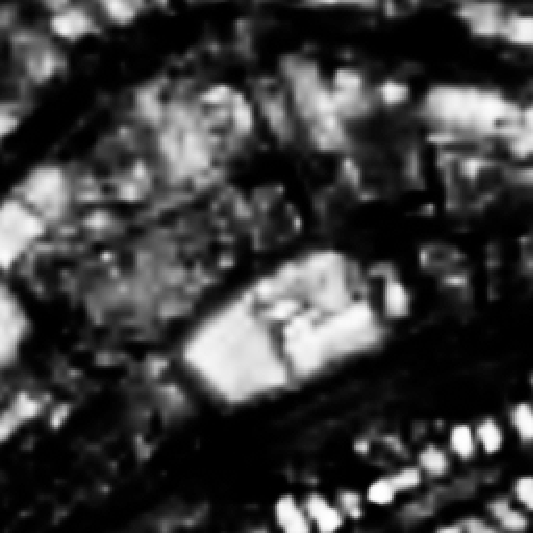
\includegraphics[width=35mm]{FCN4s-results-Prediction(f)}}
%\caption{(a)(d) Input image. (b)(e) Ground truth. (c)(f) FCN-4s prediction.}
%\label{fig:FCN4s-results}
%\end{figure}
% 
        
\subsection{Formulation}
   Our goal is to predict labelling image $\mathbf{\hat{M}}$ from a  input aerial image $\mathbf{S}$.  We directly learn a mapping from raw pixels in $\mathbf{S}$ to a true label image  $\mathbf{\tilde{M}}$ by training the whole network. Fig. \ref{fig:AGroupOfExamples} shows an example of $\mathbf{S}$, $\mathbf{\hat{M}}$, $\mathbf{\tilde{M}}$. Here we formulate our approach for building extraction. We denote our input training data set by $\mathbf{I} = \{(\mathbf{S}_{n},\mathbf{\tilde{M}}_{n}),n = 1,\ldots,\vert \mathbf{S}_n \vert \}$, where sample $\mathbf{S}_{n} = \{s_{j}^{(n)}, j = 1,\ldots,\vert \mathbf{S}_n \vert \}$ denotes the raw input image and  $\mathbf{\tilde{M}}_{n} = \{\tilde{m}_{j}^{(n)}, j = 1,\ldots,\vert \mathbf{S_n} \vert\}$, $\tilde{m}_j^{(n)} \in \{0,1\}$ denotes the corresponding ground truth binary labelling map for satellite image $\mathbf{S}_{n}$.  Taking account of each image holistically and independently, thus, we adopt the subscript $n$ for notational simplicity. Our goal is to have a network that learns features from which it is possible to produce building maps approaching the ground truth. In our image-to-image training, the loss function is computed over all pixels in a training image $\mathbf{S} = \{s_{j}, j = 1,\ldots,\vert \mathbf{S} \vert\}$ and building map $\mathbf{\tilde{M}} = \{\tilde{m}_{j}, j = 1,\ldots,\vert \mathbf{S} \vert\}$, $\tilde{m}_j \in \{0,1\}$.
For simplicity, we denote the collection of all standard network layer parameters as $\mathbf{W}$. For each pixel $j$ in a training image, the possibility that assigns it to building is denoted as $\hat{m}_j = Pr(\tilde{m}_j = 1|\mathbf{S};\mathbf{W})$. the definition of sigmoid cross-entropy loss function is shown in Eq (\ref{loss}).
\begin{equation}
	\label{loss}
    \mathcal{L} = - \frac{1}{\vert \mathbf{S} \vert} \sum_{j \in \mathbf{S}} \left[ \tilde{m}_j \log{\hat{m}_j} + (1 - \tilde{m}_j)\log{(1 - \hat{m}_j)} \right]
\end{equation}

%\begin{figure}
%\centering
%\includegraphics[width=120mm]{AGroupOfExamples}
%\caption{(a) Aerial image $\mathbf{S}$. (b) Ground truth $\mathbf{\tilde{M}}$. (c) Predicted label image $\mathbf{\hat{M}}$. }
%\label{fig:AGroupOfExamples}
%\end{figure}

\begin{figure}
\centering
\subfigure[Aerial image $\mathbf{S}$]{	
	\label{fig:AerialImage}
	\includegraphics[width=38mm]{example-aerialImage}}	
\subfigure[Ground truth $\mathbf{\tilde{M}}$]{
	\label{fig:GroundTruth}
	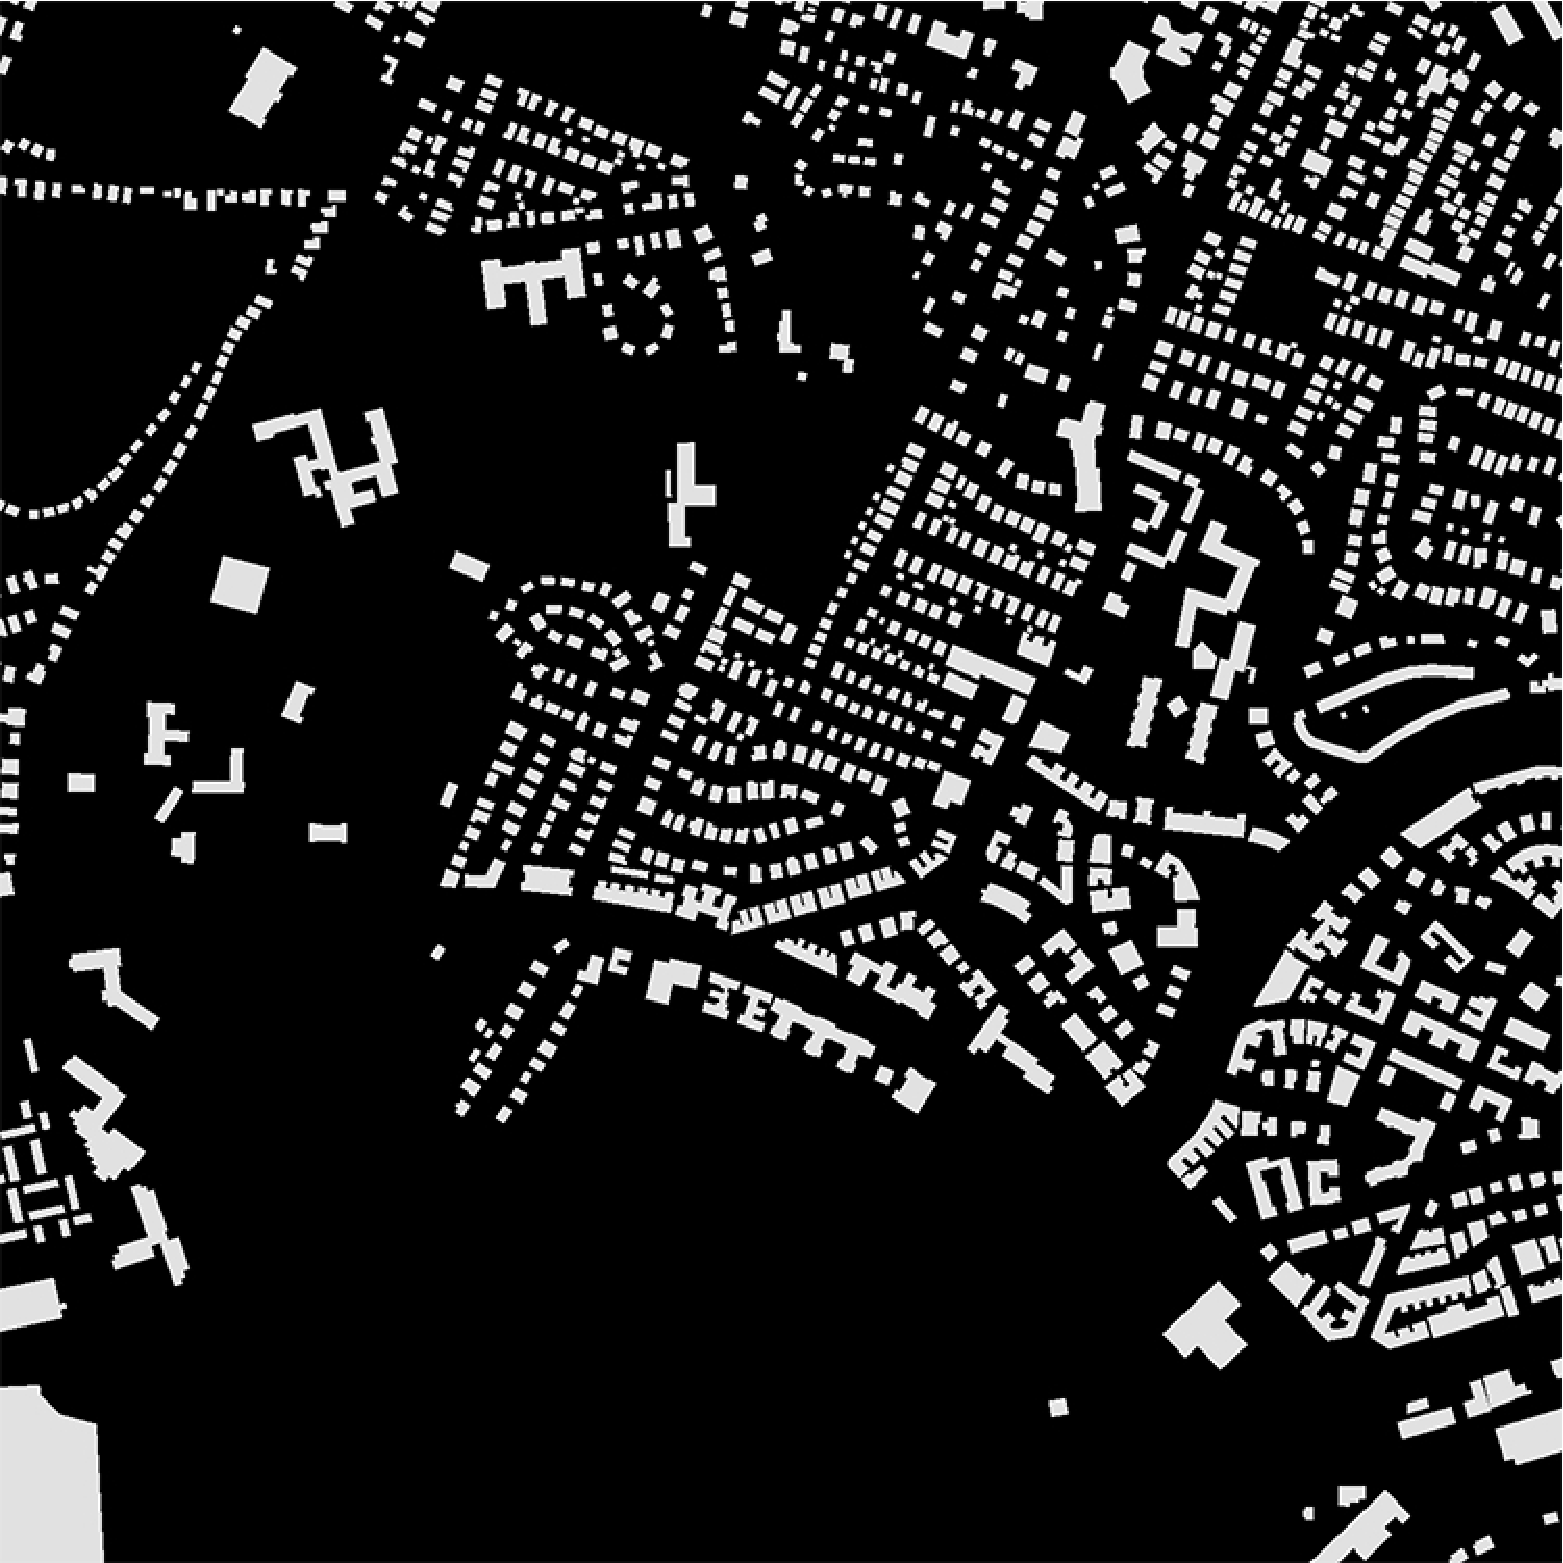
\includegraphics[width=38mm]{example-GT}}	
\subfigure[Predicted image $\mathbf{\hat{M}}$]{
	\label{fig:PredictedResutls}
	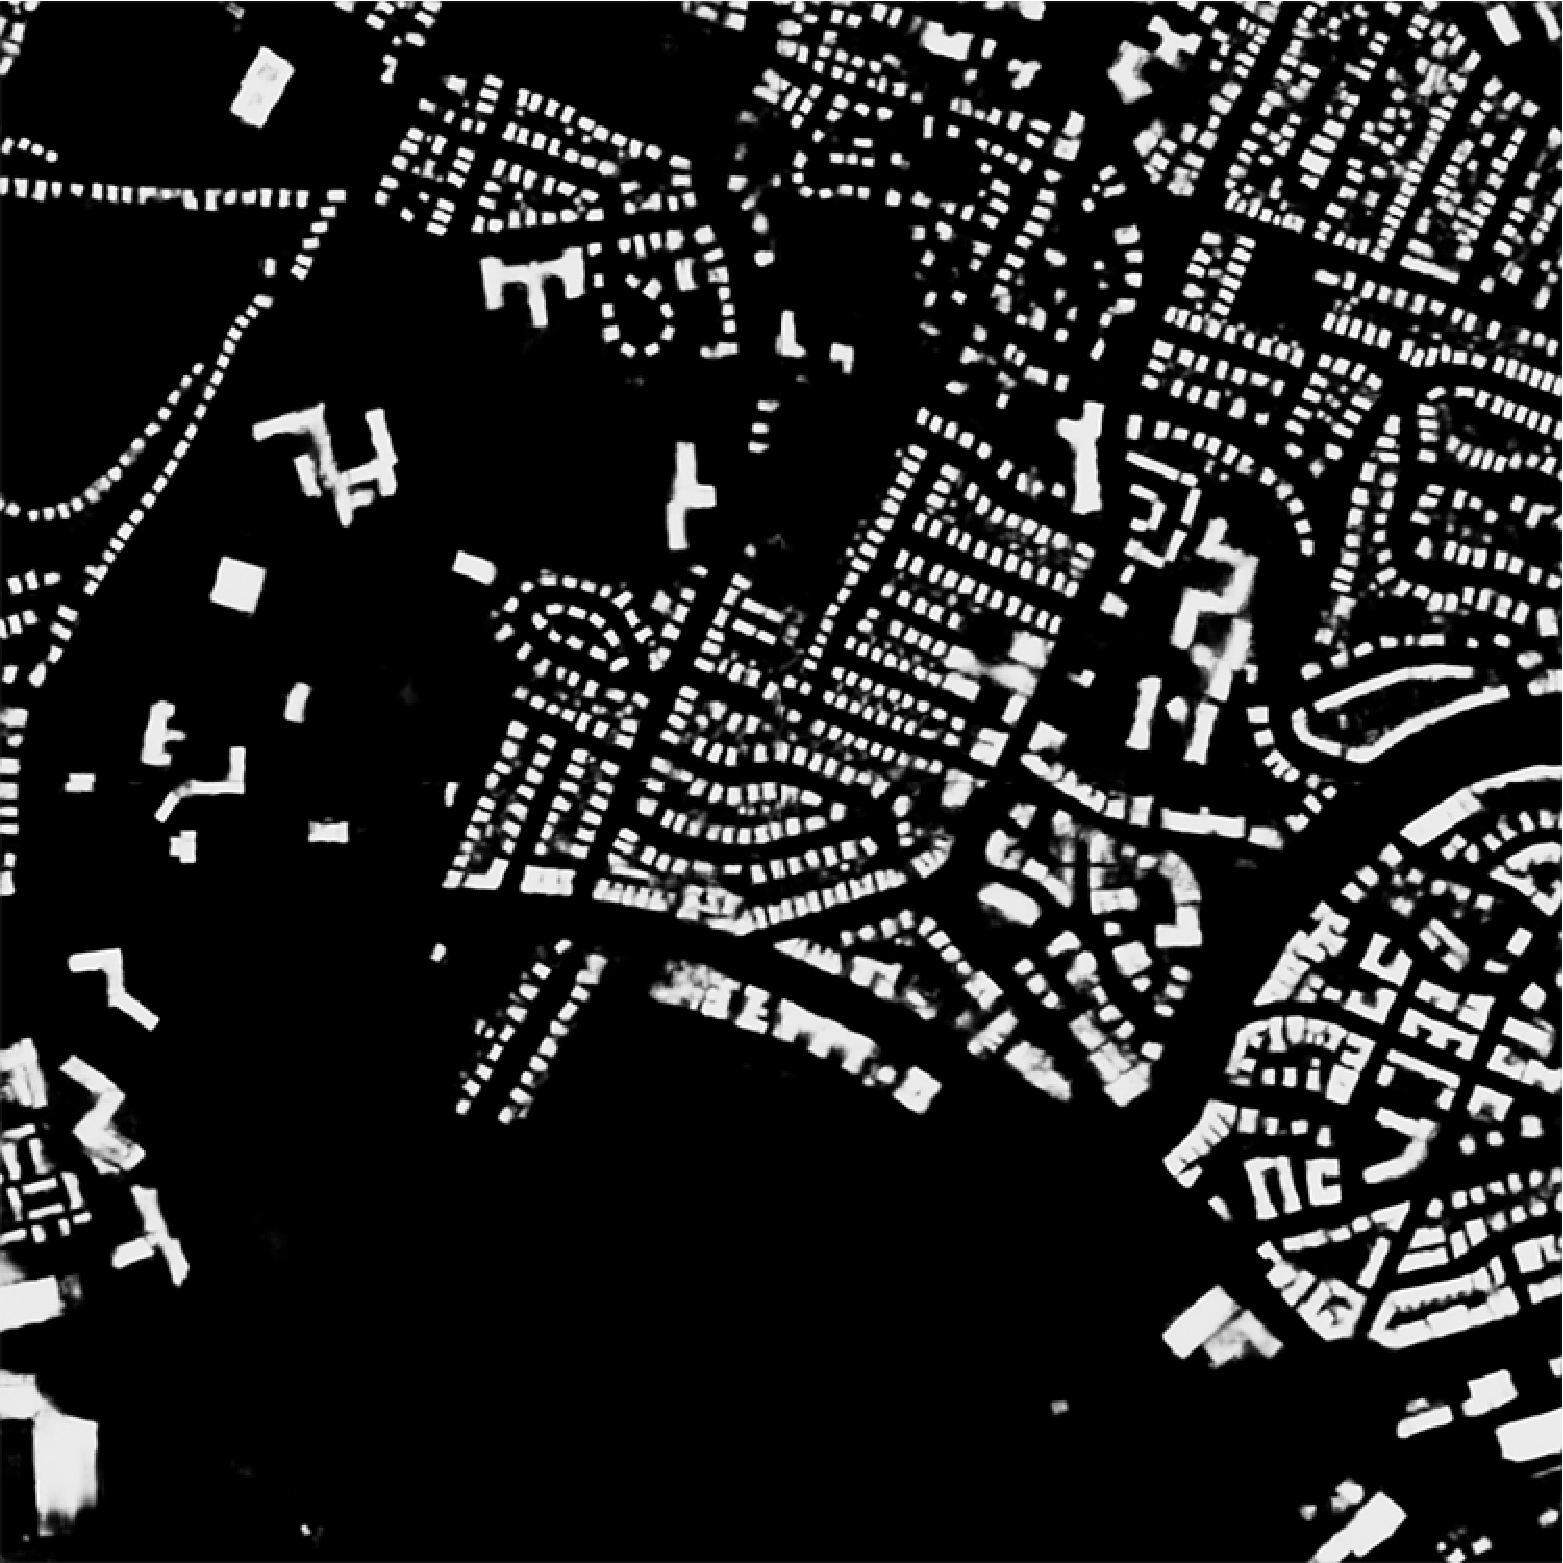
\includegraphics[width=38mm]{example-prediction}}	
\caption{ An example of the resulting predicted image.}
\label{fig:AGroupOfExamples}
\end{figure}


%===========================================================
\section{Experiments}
\label{section:experiments}
In this section, we introduce our detailed implementation and report the performance of our proposed algorithm.

\subsection{Dataset}
   In our experiments, we use Massachusetts Buildings Dataset (\textit{Mass. Buildings}) proposed by Mnih \cite{Mnih2013Machine} and publicly available on website \url{http://www.cs.toronto.e
du/~vmnih/data/}. The dataset consists of 151 aerial images of the Boston area, with each of the images being 1500$\times$1500 pixels for an area of 2.25 square kilometers. Hence, the entire dataset covers roughly 340 square kilometers. The data is split into a training set of 137 images, a test set of 10 images and a validation set of 4 images. To train the network, we create image tiles for train and validation by means of cropping entire image using a sliding window with size of 256$\times$256 pixels and stride of 64 pixels. When scanning the whole dataset, image tiles which include more than 160 white pixels are removed. After scanning, train and validation dataset include 75938 tiles and 2500 tiles with corresponding building masks. For testing, we use ten 1500$\times$1500 entire images covering area excluded from the training data. In our experiments, we find that it is benefit to improving prediction performance by means of scaling the intensity of input image into range of [0,1]. 

\subsection{Training Settings}
   The implementation of our network is based on the publicly  available \textit{Caffe} \cite{Jia2014Caffe} Library. HF-FCN is fine-tuned from an initialization with the pre-trained VGG16 Net model and trained in an end-to-end manner. It is trained using stochastic gradient descent with the following hyper-parameters, including mini-batch size (18), initial learning rate ($10^{-5}$), learning rate is divided by 10 for each 5000 iterations, momentum (0.9), weight decay (0.02), clip$\_$gradients (10000), number of training iterations (12000). We find that learned deconvolutions provide no noticeable improvements in our experiments, therefore,  lr$\_$mult is set to zero for all deconvolutional layers. Additionally, except that the pad of first convolutional layer is set to 35, others are set to 1 as the  same as VGG16 Net. It takes about six hours to train a network on a single NVIDIA Titan 12GB GPU.

\subsection{Results}
    To show the effectiveness of HF-FCN, we train and test our network on \textit{Mass. Buildings}. In order to comparing our results with previous works \cite{Mnih2013Machine,Saito2016Multiple}, we use three metrics to evaluate our results: (1) relaxed precision and recall scores ($\rho$ = 3). (2) relaxed precision and recall scores ($\rho$ = 0). (3) time cost.  The relaxed precision is defined as the fraction of detected pixels that are within $\rho$ pixels of a detected pixel, while the relaxed recall is defined as the fraction of true pixels that are within $\rho$ pixels of a detected pixel.  In  one of our experiments, the slack parameter $\rho$ is set to 3, which is the same value as used in \cite{Mnih2013Machine,Saito2016Multiple}. Compared relaxed precision-recall curves are shown in  Fig. \ref{fig:relaxedcurve}. In order to evaluate our results more strictly, we set slack parameter $\rho$ as 0, that is to say, it becomes a standard precision and recall scores. Compared standard precision-recall curves are shown in  Fig. \ref{fig:standardcurve}. Additionally, time cost is another important index to evaluate system performance. We calculate the mean time of processing ten test images in the same computer using the same program. Table \ref{tab:PerformanceComparision} shows that our method is able to not only significantly improve the performance, but dramatically decrease the time cost. 
      
\begin{figure}
\centering
\subfigure[Slack parameter $\rho$ = 3]{	
	\label{fig:relaxedcurve}
	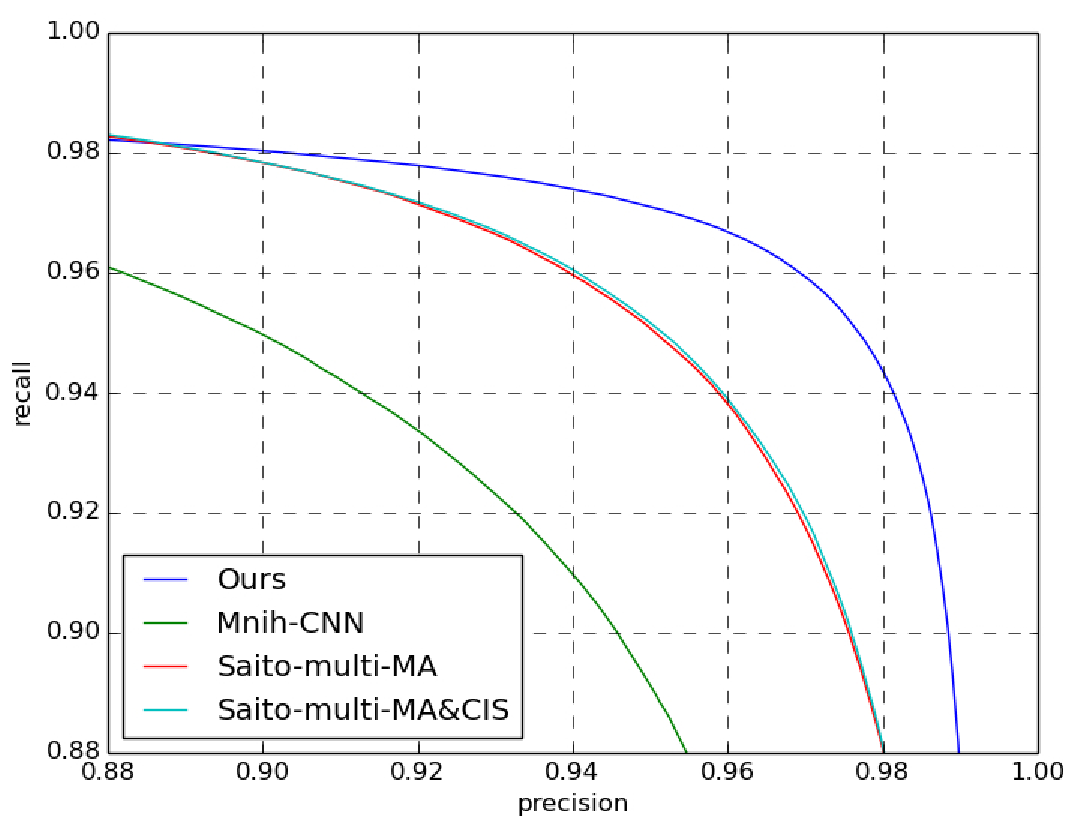
\includegraphics[width=59mm]{PrecisionRecallCurve_3}}
\subfigure[Slack parameter $\rho$ = 0]{
	\label{fig:standardcurve}
	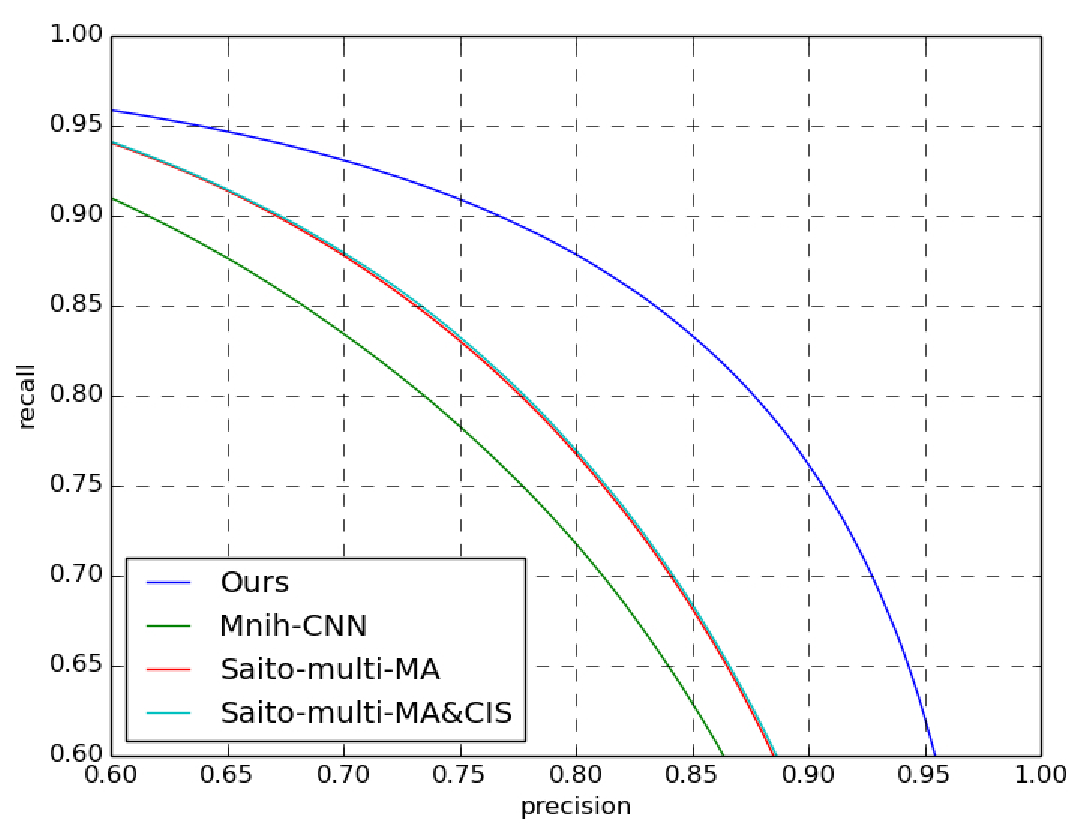
\includegraphics[width=59mm]{PrecisionRecallCurve_0}}
\caption{Two relaxed precision-recall curves}
\label{fig:}
\end{figure}
 
    \begin{table} 
    \centering
	\caption{Performance is compared with \cite{Mnih2013Machine,Saito2016Multiple}. Recall here  means recall at breakeven points. Time is computed in the same computer with a single NVIDIA Titan 12GB GPU.}
	\begin{tabular}{L{38mm}C{26mm}C{26mm}C{26mm}}     
	\toprule
	& Recall ($\rho$ = 3) & Recall ($\rho$ = 0)& Time (s)\\
	\midrule
	Mnih-CNN \cite{Mnih2013Machine} & 0.9271 & 0.7661 & 8.70  \\ 
	Mnih-CNN+CRF \cite{Mnih2013Machine} & 0.9282 & 0.7638 & 26.60\\ 
	Saito-multi-MA \cite{Saito2016Multiple} & 0.9503 & 0.7873 & 67.72 \\
	Saito-multi-MA$\&$CIS \cite{Saito2016Multiple} & 0.9509 & 0.7872 & 67.84 \\
	Ours (HF-FCN) & $\bm{0.9643}$ & $\bm{0.8424}$ & $\bm{1.07}$\\
	\bottomrule
	\end{tabular}
	\label{tab:PerformanceComparision}
	\end{table}  
 
 	 
\begin{figure}
\centering
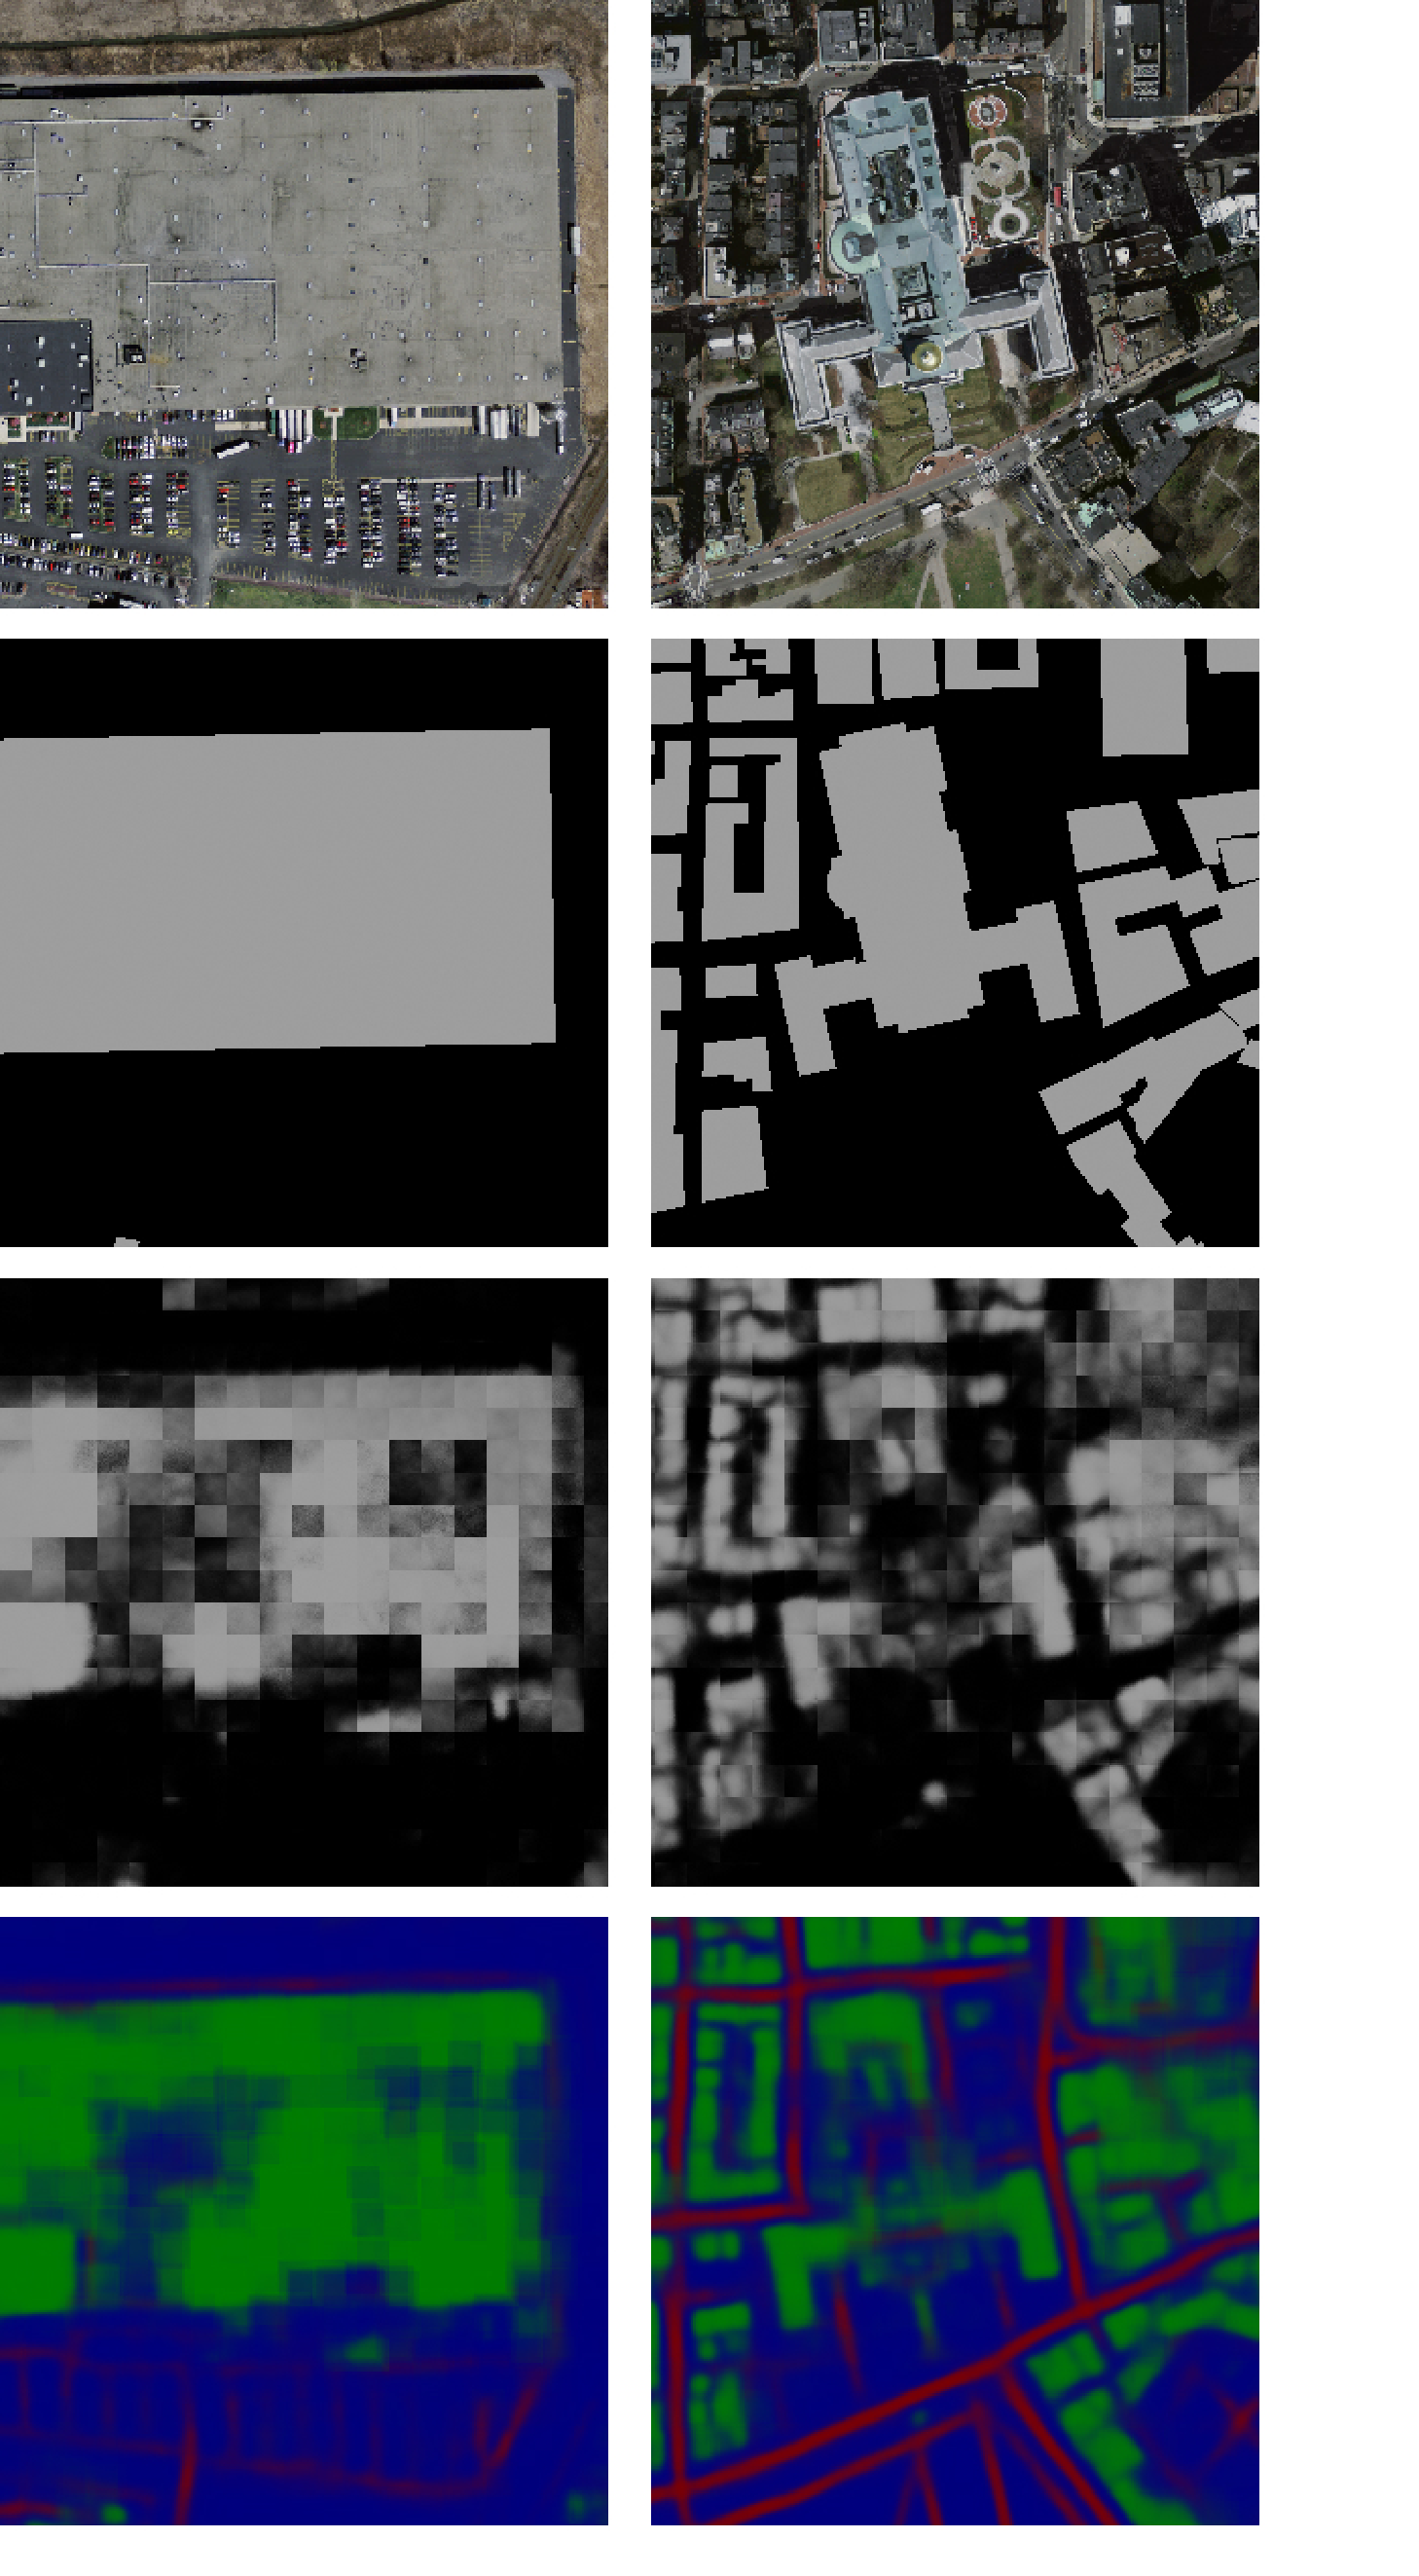
\includegraphics[width=110mm]{ComparedResults}
\caption{(a) Input images. (b) Results of Mnih-CNN+CRF \cite{Mnih2013Machine}. (c) Results of Saito-multi-MA$\&$CIS \cite{Saito2016Multiple}. (d) Our results. 
Correct results (TP) are shown in green, false positives (FP) are shown in blue, and false negatives (FN) are shown in red.}
\label{fig:ComparedResults}
\end{figure} 
    
 
  To prove our network having strong ability in extracting buildings with variant appearances, arbitrary sizes, occlusions, we perform  further evaluation. We crop seven 256$\times$256 image patches that have buildings with variant appearances or occlusions from test image of \textit{Mass. Buildings}. And then, we directly crop corresponding predictions from predicted images  generated by three models (Mnih-CNN+CRF \cite{Mnih2013Machine}, Saito-multi-MA$\&$CIS \cite{Saito2016Multiple} and ours). Here, we binarize the probability map using a threshold of 0.5. Seven groups of example are shown in Fig. \ref{fig:ComparedResults}. In addition, Table \ref{tab:ComparedResultsRecall} shows the resulting recalls at breakeven points of standard precision recall curve for each patches. 
 

	\begin{table} 
    \centering
	\caption{Recall at selected region of the test images}
	\begin{tabular}{L{38mm}*{9}{C{9mm}}}     
	\toprule
	Image ID & 01 & 02 & 03 &04 &05 & 06 &07 & mean\\
	\midrule
	Mnih-CNN+CRF \cite{Mnih2013Machine} & 0.784 & 0.869 & 0.769 & 0.653 & 0.893 & 0.764 & 0.800 & 0.784\\
	Saito-multi-MA$\&$CIS  \cite{Saito2016Multiple} & 0.773 & 0.915 & 0.857 & 0.789 & 0.945 & 0.773 &0.830 & 0.851\\
	Ours (HF-FCN) & $\bm{0.874}$ & $\bm{0.964}$  & $\bm{0.899}$ & $\bm{0.901}$ & $\bm{0.986}$ & $\bm{0.840}$ &  $\bm{0.851}$ & $\bm{0.911}$\\
	\bottomrule
	\end{tabular}
	\label{tab:ComparedResultsRecall}
	\end{table} 
 	 

%===========================================================
\section{Conclusions}
\label{section:conclusions}
   In  this article, we propose a improved fully convolutional network which is strongly capable of extracting buildings with arbitrary sizes, variant appearances or occlusions without any post-processing. Meanwhile, it further improves the overall accuracy. The network can take arbitrary-size image as input as long as GPU memory allowed. Compared with patch-based methods, there is no need to label a whole image by cropping the image into small patches. As consequence, inconsistant border caused by cropped would not occurred in our system. Though some effective techniques, such as model average and conditional random field, can improve the performance further, 
time cost is increased by several times.  While in our system, elapsed time is tremendously decreased. On the other hand, we demonstrate that our network  is generally adapt to various types of aerial scenes selected from real-world data. Furthermore, our architecture can be easily extended to extract multi-objects in remote sensing imagery. Consequently, we believe that our technique potentially provides a generic solution to understand complex aerial scenes.
	
%HF-FCN provides a strong ability to extracting building rooftops even with significantly variant appearancess and severely occlusions   Meanwhile, it further improves the overall accuracy than \cite{Mnih2013Machine}\cite{Saito2016Multiple}. Compared with patch based methods \cite{Mnih2013Machine}\cite{Saito2016Multiple}, HF-FCN takes whole images as inputs without cropping or warping them to a fixed size and directly outputs segmentation maps by one pass of forward propagation. 
%===========================================================
\bibliographystyle{splncs}
\bibliography{egbib}

%this would normally be the end of your paper, but you may also have an appendix
%within the given limit of number of pages
\end{document}
